\documentclass[../main.tex]{subfiles}
\begin{document}

\chapter{Grundlagen}
\label{basics}

	\section{Virtualisierung}
  \label{introVirt}
		Der Einsatz von Virtualisierung bietet vielfältige, attraktive Eigenschaften für \acrshort{IT}-Unternehmen. In der folgenden Auflistung sind einige Problemfaktoren und Anforderungen an Rechenzentren und darin laufender Software zusammengefasst, die alle durch Virtualisierungslösungen adressiert werden können \cite[S.1]{bsiVirt}\cite[S.662,672f.]{tanenbaumOS}\cite[S.299]{mandlOS}.

		\vspace{0.5cm}
		\begin{table}[h!]
			\begin{centering}
			\begin{tabularx}{\textwidth}{>{\hsize=1\hsize}X|>{\hsize=1\hsize}X}
				\hline
				\textbf{Herausforderung} & \textbf{Lösungsansatz mithilfe von Virtualisierung} \\
				\hline
				Effizienter Betrieb von Rechenzentren
				& Einsparungen bei Anschaffung von Hardware und Lizenzen. Bessere Auslastung physischer Ressourcen. \\
				\hline
				Skalierbarkeit und Redundanz von Diensten
				& Virtuelle Systeme sind i.d.R. hardwareunabhängig, portierbar und reproduzierbar. Damit sind Skalierbarkeit und Redundanz realisierbar. \\
				\hline
				Realisierung von Multi-Tenancy-Umgebungen
				& Abgrenzung von Kundeninstanzen durch Isolierung. \\
				\hline
				Realisierung bestimmter Architekturen, wie z.B. einer \emph{\gls{DreiTierArchitektur}}
				& Reproduzierbarkeit, flexible Koppelung mit unabhängigen Netzwerkfunktionen von virtuellen Systemen. \\
				\hline
				Unterstützung von Legacy-Code und mehrerer Software-Versionen
				& Gute Migrationseigenschaften, hoher Grad an Kompatibilität, Unabhängigkeit von Hardware und Betriebssystemen z.B. mit \emph{\glspl{VirtualAppliance}} möglich.\\
				\hline
				Administration und Wartbarkeit
				& Zentralisiert für physische und virtuelle Systeme möglich, auch mit Unterstützung von Tools. Senkung von Administrationskosten \cite[S.1]{bsiVirt}\cite[S.661]{tanenbaumOS}. \\
				\hline
			\end{tabularx}
			\vspace{0.5cm}
			\caption{Herausforderungen und Lösungsansätze durch Virtualisierung in Rechenzentren.}
			\label{tab:virtAdvantages}
			\end{centering}
		\end{table}

		%Wie in Tabelle \ref{tab:virtAdvantages} stichpunktartig zusammengefasst ist, bietet der Einsatz von serverseitiger Virtualisierung eine Reihe von Vorteilen, die ein rein physischer Betrieb von Servern nicht in dem Maß bieten kann.
		Die Virtualisierungsmerkmale aus Tabelle \ref{tab:virtAdvantages} eröffneten IT-Unternehmen neue Geschäftsmodelle, auf denen der Erfolg von heutigen Cloud-Anbietern wie \emph{Amazon}, \emph{Google} und \emph{Microsoft} beruht. Selbst einhergehende Nachteile der Virtualisierung, wie z.B. Leistungsverluste und in dieser Arbeit untersuchte Sicherheitsrisiken, scheinen, basierend auf dem Erfolg genannter Anbieter, nicht ins Gewicht zu fallen.

		%Aus technischer Sicht, werden bei der in dieser Arbeit relevanten Virtualisierung ein oder mehrere virtuelle Systeme auf einem physischen System betrieben \cite[S.8]{advancedServerVirt}.
    %Bei der Virtualisierung, deren Anfänge sich auf IBM-Forschungsprojekte von 1964 zurückführen lassen, werden ein oder mehrere virtuelle Systeme auf einem physischen System betrieben \cite[S.8]{advancedServerVirt}.
		%Diese Systeme können kombiniert in Rechenzentren als eine Serverinfrastruktur betrachtet werden. In dieser können physische und virtuelle Komponenten gemeinsam administriert werden \cite[S.661]{tanenbaumOS}.

		Die Absicht der in dieser Arbeit relevanten Virtualisierung ist es, die in Tabelle \ref{tab:virtAdvantages} genannten Vorteile zu erreichen, indem ein System in ein oder mehrere Systeme aufgeteilt wird. Per Definition besteht ein System aus allen Ressourcen, die eine Anwendung benötigt, um fehlerfrei laufen zu können \cite[S.106]{tanenbaumOS}. Technisch gesehen beinhaltet es ein Betriebssystem und zugehörige Peripheriegeräte, wie z.B. eine Netzwerkkarte.

		Systeme können auf mehrere Arten unterschieden werden, z.B. in physische und virtuelle Systeme:

		\begin{itemize}
			\item \textbf{Physisches System}: System, das direkt auf der Hardware ausgeführt wird.
			\item \textbf{Virtuelles System}: System, das virtuell innerhalb eines anderen physischen oder virtuellen Systems ausgeführt wird.
		\end{itemize}

		Eine weitere Unterscheidung trennt Systeme nach ihrer Rolle:

		\begin{itemize}
			\item \textbf{Hostsystem}: Physisches oder virtuelles System, das virtuelle Systeme (Gastsysteme) betreibt. In einem Hostsystem läuft eine Virtualisierungssoftware wie z.B. Docker, die die Instanziierung von Gastsystemem ermöglicht.\\
			\textbf{Beispiel}: Linux-Distribution mit Docker-Installation
			\item \textbf{Gastsystem}: Virtuelles System, das im Kontext eines übergeordneten Hostsystems läuft.\\
			\textbf{Beispiel}: Docker-Container
		\end{itemize}


		%Virtuelle und physische Systeme können dabei als minimale oder vollständige Betriebssysteme vorliegen. Systeme können in Rechenzentren eine Serverinfrastruktur bilden, in der virtuelle als auch physische Komponenten gemeinsam verwaltet werden .

		%Die Unterscheidung in virtuelle und physische Systeme ist nicht von Bedeutung, wenn allein der Begriff \glqq{}System\grqq{} aufgeführt ist. %Wenn die Abgrenzung minimaler Betriebssysteme von vollständigen Betriebssystemen notwendig ist, wird das jeweilige Attribut an entsprechender Stelle verwendet. Standardmäßig ist allgemein von einem (Betriebs-)System die Rede.
		%Per Definition in dieser Arbeit, besteht ein System aus einem Betriebssystem und zugehörigen Peripheriegeräte, wie z.B. einer Netzwerkkarte.

		%Ein System, das mehrere virtuelle Systeme betreibt, wird allgemein als Host oder Hostsystem bezeichnet. Systeme, die einzeln oder parallel virtualisiert auf einem solchen Host laufen, werden als (virtuelle) Gastsysteme bezeichnet.

		Das Hostsystem ist nicht mit einem Host im Sinne der Netzwerktechnik zu verwechseln. Der Host eines Netzwerks meint einen kommunikationsfähigen Netzwerkknoten. Sowohl Host- als auch Gastsysteme können Hosts eines Netzwerks darstellen.

		%Der Begriff des Hosts ist abzugrenzen von der Bedeutung eines Hosts in der Netzwerktechnik. In der Netzwerktechnik ist damit ein kommunikationsfähiger Netzwerkknoten gemeint. Ein in dieser Arbeit erwähnter Host meint das Hostsystem, welches Gastsysteme, mithilfe von Virtualisierungsprogrammen wie Docker, startet und stoppt.

		%Das Hostsystem kann physischer oder virtueller Natur sein:
		%\begin{itemize}
			%\item \textbf{Physischer Host}: Hostsystem, das Gastsysteme verwaltet und selbst direkt (nativ) auf der Hardware läuft.
			%\item \textbf{Virtueller Host}: Hostsystem, das Gastsysteme verwaltet und selbst als Gastsystem eines übergeordneten Hosts existiert.
		%\end{itemize}

		%Im Vergleich zu dieser Unterscheidung, ist ein Gastsystem immer virtueller Natur.
		%Die Einheit eines physischen Hosts inklusive aller darin betriebenen virtuellen Systeme, wird in dieser Arbeit als Maschine bezeichnet.


		Wie diese Definition andeuten, sind virtuelle Verschachtelungen innerhalb eines physischen Hostsystems möglich und auch in der Praxis begrenzt sinnvoll. Beispielsweise kann in einem Rechenzentrum jeder physische Host mehreren Kunden dienen, indem jedem Kunden ein Gastsystem auf diesem physischen Host zugewiesen wird. Ein Kunde kann dieses Gastsystem wiederum als virtuelles Hostsystem betreiben, das jede Anwendung des Kunden in einem eigenen, neuen Gastsystem virtualisiert. Wie diese Trennung von Kunden und Kundenanwendungen zeigt, eignet sich eine Verschachtelung der virtuellen Systeme zur Abbildung von organisatorischen und operationalen Strukturen.

		Gastsysteme existieren in zwei Ausprägungen:
		\begin{itemize}
			\item \textbf{Hypervisorbasierte Gastsysteme:} Ein Gastsystem, das durch einen Hypervisor des übergeordneten Hostsystems instanziiert wird. Ein hypervisorbasiertes Gastsysteme wird als virtuelle Maschine, kurz \acrshort{VM}, bezeichnet.
			\item \textbf{Containerbasierte Gastsysteme:} Ein Gastsystem, das von einer auf dem Hostsystem installierten Containertechnologie erstellt wurde. Ein containerbasiertes Gastsystem wird abgekürzt als Container bezeichnet.
		\end{itemize}

		Beide Ausprägungen erwecken aus Sicht des Gastsystems den Eindruck, dass ein alleinstehendes, direkt auf der Hardware laufendes System ausgeführt wird.	Die Art und Weise, wie beide Arten Funktionen eines übergeordneten Hostsystems abstrahieren, weist Unterschiede auf, die in Abschnitt \ref{introVirtHypervisor} und \ref{introVirtContainer} näher beschrieben sind.



		%Im Folgenden sind die Konzepte der Virtualisierung auf Hypervisor- und Containerbasis erklärt und in ihren ausschlaggebenden Eigenschaften gegenübergestellt.


		% TODO: cahpter 2 usage scenarios einbinden aus
		%	Evtl. auch strengere Trennung in verschiedene Vorteile von Virtualisierung.
		%		^		\cite[S.2,3]{dockerSec2}

    \subsection{Hypervisorbasierte Virtualisierung}
    \label{introVirtHypervisor}
      Im Kontext einer hypervisorbasierten Virtualisierung wird das Gastsystem eine \acrshort{VM} genannt. \acrshort{VM}s enthalten jeweils eine Umgebung, die Abstraktionen eines sogenannten Hypervisors nutzen, um Hardwareressourcen des Hostsystems zu verwenden. Der Hypervisor, auch seltener \emph{Virtual Machine Monitor} (\emph{VMM}) genannt, ist eine Software, die zwischen dem Host- und Gastsystem vermittelt und Abstraktionen des ersteren bereitstellt \cite[S.6]{dockerBook}\cite[S.2]{containerVirtPerformance}\cite[S.105]{tanenbaumOS}.

      % Auf dieser Art von Systemen laufen eine oder mehrere VMs unabhängig voneinander auf physischer Hardware (in der englischen Literatur auch "bare metal" genannt). Der Hypervisor, der auch \emph{Virtual Machine Monitor} (\emph{VMM}) genannt wird \cite[S.2]{containerVirtPerformance}, nimmt dabei die Rolle eines Vermittlers zwischen Host-OS und Gast-OS ein \cite[S.6]{dockerBook} und abstrahiert dem Gast das komplette Funktionsset des Hosts. \cite[S.2]{dockerSec1}.

      Durch diese Technik läuft in jeder \acrshort{VM} ein eigenes Betriebssystem, das von solchen anderer \acrshort{VM}s isoliert läuft. Durch die Abstraktion des zwischenliegenden Hypervisors ist es möglich, mehrere unterschiedliche Gastsysteme auf einem Hostsystem auszuführen \cite[S.2]{containerVirtPerformance}\cite[S.106]{tanenbaumOS}.

			Trotz der in Tabelle \ref{tab:virtAdvantages} aufgeführten effizienteren Ressourcennutzung im Rahmen von Virtualisierungstechniken, stehen Hypervisor heute unter dem Ruf ineffizient zu arbeiten. Dieser größte Kritikpunkt der genannten Virtualisierungsmethode, lässt sich auf den Erfolg der containerbasierten Virtualisierung zurückführen, die, wie in Kapitel \ref{introVirtContainer} weiter ausgeführt, weniger Leistungsverluste erzeugt.

			Bekannte hypervisorbasierte Technologien sind die kommerziellen Vertreter \emph{ESXi} der Firma \emph{VMware} und \emph{Hyper-V} von \emph{Mircosoft}, sowie die Open-Source-Vertreter \emph{Xen} und \emph{KVM} \cite[S.1]{dockerLXCKub}.
      %TODO: mehr Quellen

      Generell werden Hypervisor in Typ-1 und Typ-2 unterschieden. Der Aufbau beider Typen ist in den folgenden zwei Abschnitten dargestellt.

			%Unter beiden Typen wird jedoch eine vollständige Abstraktion von Ressourcen des Hostsystems erzielt. VMs werden in beiden Fällen wie reale Systeme gestartet und unterliegen der Illusion als alleiniges, natives System zu operieren \cite[S.665f.]{tanenbaumOS}.

			\subsubsection{Hypervisor Typ-1}
				Der Typ-1 Hypervisor operiert direkt auf der Hardware und stellt ein minimales, speziell für den Betrieb von VMs ausgelegtes Betriebssystem dar. Die Architektur eines solchen Hypervisors ist in \fig \ref{fig:intro_hypervisor1} abgebildet.

				\begin{figure}[h]
	          \centering
	          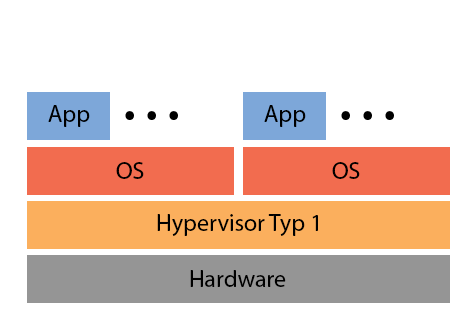
\includegraphics[width=0.7\textwidth]{./images/intro_hypervisor1.png}
	          \caption{Architektur eines Systems mit Typ-1 Hypervisor (eigene Abbildung auf der Basis von \cite[S.107]{tanenbaumOS}).}
	          \label{fig:intro_hypervisor1}
	      \end{figure}

				%Dessen Aufgabe ist es, Kopien der realen Hardware bereitzustellen, die von VMs genutzt werden können. Wenn in der VM ein Befehl ausgeführt, wird dieser an den Hypervisor weitergeleitet, der den Befehl untersucht. Handelt es sich um einen Befehl des Betriebssystem der VM, wird dieser auf dem Typ-1 Hypervisor ausgeführt. Im Fall eines Aufrufs einer Anwendung innerhalb der VM, emuliert der Hypervisor für diesen Aufruf die Aktion der realen Hardware \cite[S.663ff.]{tanenbaumOS}.

			\subsubsection{Hypervisor Typ-2}
				Ein Typ-2 Hypervisor arbeitet nicht direkt auf der Hardware, sondern innerhalb eines Hostbetriebssystems, das selbst wiederum direkt auf die Hardware zugreift. Die Architektur dieser Art von Hypervisor ist in \fig \ref{fig:intro_hypervisor2} dargestellt.

				\begin{figure}[h]
	          \centering
	          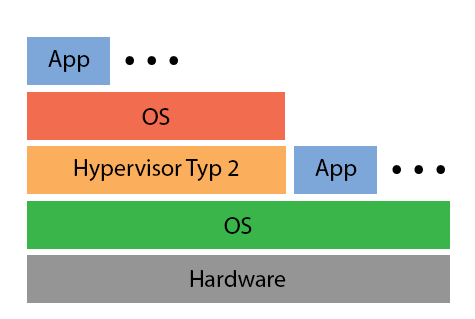
\includegraphics[width=0.7\textwidth]{./images/intro_hypervisor2.png}
	          \caption{Architektur eines Systems mit Typ-2 Hypervisor (eigene Abbildung auf der Basis von \cite[S.107]{tanenbaumOS}).}
	          \label{fig:intro_hypervisor2}
	      \end{figure}

				In dieser Variante ist der Hypervisor eine gewöhnliche Anwendung, die auf dem Hostsystem ausgeführt wird.

				%Falls ein Aufruf aus dem Gastsystem einen Hardwarezugriff benötigt, wird die Hardware - wie auch bei Typ-1 - emuliert. Erfordert ein Aufruf keinen Hardwarezugriff, wird dieser innerhalb des Gastsystems verarbeitet und verlässt dieses nicht.

				Im Durchschnitt führt die zusätzliche Softwareschicht des Hypervisors Typ-2 trotz verschiedener Optimierungsmöglichkeiten, z.B. der sogenannten Paravirtualisierung, zu höheren Leistungseinbußen wie jenen unter Typ-1 \cite[S.666f.]{tanenbaumOS}.

				%Die Aufrufe eines in dieser Anwendung installierten Betriebssystems, werden mithilfe einer sogenannten Binärübersetzung in Prozeduren des Hypervisors übersetzt, sofern der initiierte Befehl einen Hardwarezugriff verlangt.

				%Hypervisor-Prozeduren dienen auch hier wieder zur Hardwareemulation, die auf dem Hostsystem ausgeführt werden. Erfordern Teile der Gastanwendung keinen Hardwarezugriff, werden diese im Gast selbst verarbeitet und verlassen diesen nicht.

			%Unter beiden Typen wird jedoch eine vollständige Abstraktion von Hostressourcen erzielt. VMs werden in beiden Fällen wie reale Systeme gestartet und unterliegen der Illusion als alleiniges, natives System zu operieren \cite[S.665f.]{tanenbaumOS}. Es existieren dennoch Anhaltspunkte für Gastsysteme und dessen Anwendungen, um zu bestimmen, ob sie sich in einer physischen oder virtuellen Umgebung befinden.
			% Quelle erwaehen von http://serverfault.com/questions/65718/vmware-linux-server-how-can-you-tell-if-you-are-a-vm-or-real-hardware






    \subsection{Containerbasierte Virtualisierung}
    \label{introVirtContainer}
      Die containerbasierte Virtualisierung wird vorrangig als leichtgewichtige Alternative zu der hypervisorgestützen Virtualisierung gesehen\cite[S.2]{containerVirtPerformance}.

			Während ein Hypervisor für jede \acrshort{VM} ein vollständiges System abstrahiert, werden für Container direkt Funktionen des Hostsystems über \emph{\glspl{SystemCall}} zur Verfügung gestellt. Container kommunizieren über diese direkt mit dem Hostsystem und teilen sich dessen Kernel \cite[S.6f.]{dockerBook}\cite[S.2]{containerVirtPerformance}. Ein Hypervisor wird in diesem Ansatz nicht benötigt. Vielmehr wird das Hostsystem und dessen Ressourcen partitioniert, sodass mehrere virtuelle, voneinander isolierte Container betrieben werden können \cite[S.3]{dockerSecIntro}\cite[S.1]{dockerSec2}.

			Die Isolation basiert auf dem Konzept von Kontexten, die unter Linux \emph{Namespaces} genannt werden. Diese, sowie \emph{Control Groups}, die für das Ressourcenmanagement verantwortlich sind, werden in den Kapiteln \ref{secIsolierung} und \ref{secCgroups} genauer betrachtet \cite[S.4]{dockerSecIntro}.

			% Need to link acronym and glossary entry for chroot separately here, so cross references are generated properly
      Container sind durch den Unix-Befehl \texttt{\acrshort{chroot}} inspiriert, der schon seit 1979 im Linux-Kernel integriert ist. In \emph{FreeBSD} wurde eine erweiterte Variante von \texttt{\gls{chrootGlossary}} verwendet, um sogenannte \emph{Jails} (\emph{FreeBSD}-spezifischer Begriff) umzusetzen \cite{jails}. In \emph{Solaris}, ein von dem Unternehmen \emph{Oracle} entwickeltes Betriebssystem für Servervirtualisierungen \cite{solaris}, wurde dieser Mechanismus in Form von \emph{Zones} (\emph{Solaris}-spezifischer Begriff) \cite{zones} weiter verbessert. Auch proprietäre Lösungen von \emph{HP} und \emph{IBM} erschienen auf dem Markt \cite[S.2]{dockerLXCKub}.

			Durch die kontinuierliche Weiterentwicklung von Containern in den letzten Jahren, können diese heutzutage laut \cite[S.7]{dockerBook} als vollwertige Systeme betrachtet werden, nicht mehr als - wie ursprünglich vorgesehen - reine Ausführungsumgebungen auf Basis von \texttt{chroot}.

			Dieses Design hat einen entscheidenen Nachteil gegenüber dem Hypervisormodell, der auch Docker betrifft: das Betriebssystem im Hostsystem muss Linux-basiert sein \cite[S.6]{dockerBook}. Allerdings streben \emph{Docker} und \emph{Microsoft} eine native Docker-Lösung für \emph{Microsoft Windows Server 2016} an \cite{dockerWindowsSupport}.
			%Durch das \emph{Open Container Project} (siehe Kapitel \ref{dockerContainerformate}) ist es dem Unterstützer \emph{Microsoft} nun möglich, den Windows-Kernel für das neue standardisierte Containerformat vorzubereiten .
			% Mittels github.com/mircrosoft/hcsshim

			Ein großer Vorteil jedoch, der sich durch das schlanke Design von Containern ergibt, ist eine fast native Performance dieser \cite[S.1]{containerVirtPerformance}, da der Hypervisor in diesem Modell nicht existiert. Unter dem Gesichtspunkt der Rechenleistung, kommt es bei Containerlösungen im Durchschnitt zu einem Verlust von ca. 4\%, wenn dieser mit der nativen Leistung derselben Hardwarekonfiguration verglichen wird \cite[S.4]{containerVirtPerformance}\cite[S.5]{IBMcontVMcomparison}. In traditionellen Virtualisierungen beansprucht der Hypervisor allein etwa 10-20\% der Hostkapazität \cite[S.2]{dockerIntroIEEE}\cite[S.5]{IBMcontVMcomparison}. Ein Benchmarktest, der den Durchsatz (Operationen pro Sekunde) einer \emph{VoltDB}-Konfiguration \cite{voltdb} auf hypervisor- und containerbasierten Systemen gegenüberstellt, kommt zu dem Ergebnis, dass Container eine fünffache Leistung aufweisen \cite[S.2f.]{voltdbBenchmark}.

			In der Praxis ermöglichen diese Verhältnisse eine hohe Dichte an Containern und führen zu einer besseren Resourcenausnutzung \cite[S.7f.]{dockerBook}. Der resultierende Leistungsgewinn ist v.a. für \emph{High Performance Computing}, sowie ressourcenbeschränkte Umgebungen wie mobile Geräte und \emph{Embedded Systems}, wichtig \cite[S.1]{dockerSec2}.

      Aus dem Blickwinkel der Sicherheit kann das Fehlen eines Hypervisors kontrovers interpretiert werden: Zum einen schrumpft die Angriffsfläche des Hostsystems, da nicht das gesamte Betriebssystem virtualisiert wird \cite[S.6]{dockerBook}. Je weniger Hostsystemfunktionen virtualisiert werden, desto geringer wird auch das Sicherheitsrisiko, das eine Funktion von einem Angreifer missbraucht wird. Zum anderen ist das Konzept eines geteilten Kernels generell unsicherer, da die Sicherheitsziele hierbei durch zusätzliche Mechanismen gewahrt werden müssen.

			Die angewandten Sicherheitsmodelle und -mechanismen werden ausführlich in Kapitel \ref{secLinux} behandelt.

			%Angriffe, die von einer VM über die zusätzliche Softwareschicht eines Hypervisors das Hostsystem zum Ziel haben, sind - wie der Erfolg von Hypervisorn der letzten Jahre bestätigt - sehr schwierig durchzuführen.
			% TODO: Quelle dazu (irgendwo stand das so oder so ähnlich)
			%Deswegen werden Container als weniger sicher im Vergleich zur Hypervisor-gestützen Virtualisierung gesehen \cite[S.6]{dockerBook}. Mit welchen Sicherheitsmechanismen Container ausgerüstet sind, ist Gegenstand von Kapitel \ref{secLinux}.
			% TODO: System Calls erklaeren. Entweder in anderem Kapitel (sec) oder im Gloassar

      % TODO: Grafik für Container-based und Hypervisor-based Virtualization und deren Schichten (einmal mit, einmal ohne Hypervisor)

			Auch im Lifecycle von virtuellen Instanzen bieten Container Vorteile: Während in traditionellen \acrshort{VM}s ein Neustart Sekunden bis Minuten beansprucht, entspricht der Neustart von Containern nur einem Prozessneustart auf dem Hostsystem, der im Millisekundenbereich abgeschlossen ist \cite[S.2]{dockerLXCKub}.
			Im Fall von VMs muss das komplette Gastbetriebssystem neu gestartet werden.

	  \subsection{Einordnung Docker}
      Docker zählt zu den Technologien der containerbasierten Virtualisierung und hat seinen Ursprung in \emph{Linux Container} (\emph{LXC}), das mit Docker rundum erweitert wurde. \cite[S.7]{dockerBook}\cite[S.1]{containerVirtPerformance}\cite[S.2]{dockerLXCKub}.

      % Unbedingt Quelle containerVirtPerformance anschauen, da werden mehrere Containerloesungen miteinander verglichen.

      Docker ist wie in Kapitel \ref{introVirtContainer} zuvor erwähnt, nicht die erste containerbasierte Virtualisierungslösung. Einige ältere Containersysteme, wie z.B. \emph{Solaris Zones}, existieren bereits länger als Docker, erlangten allerdings nie die Popularität von Docker.
			%Der anhaltende Erfolg von Docker beruht jedoch überwiegend nicht auf den technischen Eigenschaften, die sich von jener der Konkurrenz wie \emph{LXC} und \emph{rkt} abheben, sondern vielmehr auf den Tools und einem effizienten Workflow, den \emph{Docker} seinen Kunden anbietet.

			% Vergleich zu lmctfy von Google oder LXC oder OpenVZ?
			% \cite[S.3]{virtVSContainer}

  \section{Sicherheitsziele in der IT}
  \label{introSecGoals}
		In der IT existieren mehrere Sicherheitsziele, die auf unterschiedliche Art und Weise erreicht werden. Je nach Anwedungsgebiet und Anforderungen werden die einzelnen Ziele unterschiedlich stark priorisiert bzw. nicht angewandt. Auch im Zusammenhang mit der Virtualisierung lassen sich die Sicherheitsziele eingrenzen, sodass in den folgenden Abschnitten nur die in dieser Arbeit relevanten Ziele aufgeführt sind.
		%Warum diese Einschränkung Sinn macht, ist im darauffolgenden Kapitel \ref{question} erklärt.
		% TODO: Warum diese Einschränkung Sinn macht, ist im darauffolgenden Kapitel \ref{question} erklärt --> SICHERGEHEN

		Grundsätzlich wird zwischen der Sicherheit von Computersystemen und Netzwerken unterschieden. Die Virtualisierung auf Containerbasis ist vorrangig ein Element von Computersystemen und ist von den Netzwerken, an die Systeme angeschlossen sind, zunächst unabhängig. Aus diesem Grund sind in diesem Kapitel nur die von Tanenbaum definierten Sicherheitsziele definiert \cite[S.712f.]{tanenbaumOS}.

		% TODO: jeweils mit Quelle belegen.
		% https://tools.ietf.org/html/rfc1704
		% https://tools.ietf.org/html/rfc3552
		% S.26 patricks diplomarbeit
		% https://tools.ietf.org/html/rfc2196

		% Evtl. Unterschiedung in Kommunikationssicherheit und Systemsicherheit vornehmen

		% klassische Sicherheitsanforderungen, die im Kontext von SELinux relevant sind:
		%		Vertraulichkeit, Systemintegrität, "Principle of Least Privilege"

		% TODO: Auf NIST verweisen und server security principles


    \subsection{Vertraulichkeit}
			Die Vertraulichkeit steht für das Konzept von Geheimhaltung. In Computersystemen können die z.B. in Kapitel \ref{secLinux} beschriebenen Mechanismen von Linux aktiviert werden, um eine bestimmte Information vor unauthorisierten Zugriffen zu schützen. Somit haben ausschließlich Befugte Zugang zu kritischen Information. In einem Multi-Tenancy-System ist es beispielsweise notwendig, Kundeninformationen von unberechtigten Nutzern geheimzuhalten.

    \subsection{Integrität}
			Unter Integrität versteht man die Zusicherung, dass bestimmte Daten original und vollständig vorliegen, sowie nachweisbar nicht manipuliert wurden. Ein Sicherheitsmechanismus, der die Integrität sicherstellen soll, bewirkt z.B., dass es nur dem Besitzer einer Datei möglich ist, diese zu modifizieren. In Multi-Tenancy-Systemen muss beispielsweise gewährleistet werden, dass die Daten der einzelnen Kunden geschützt werden und kein Kunde die Integrität von Daten anderen Kunden verletzen kann.

    \subsection{Verfügbarkeit}
			Die Verfügbarkeit bezeichnet die Eigenschaft eines Systems, Anfragen jederzeit zu verarbeiten und andere Systeme nicht negativ zu beeinflussen. Angriffe gegen die Verfügbarkeit werden als \gls{DenialOfService}-Angriffe bezeichnet. Beispielsweise muss in Multi-Tenancy-Systemen sichergestellt sein, dass ein Kunde nicht die Ressourcen anderer Kunden erschöpft.

		\subsection{Authentizität}
			Authentizität bezeichnet die Sicherstellung der Echtheit und Überprüfbarkeit. Es wird die Identifikation eines Nutzers im Rahmen einer Authentifizierung auf Echtheit geprüft. Kommt z.B. in Client-Server-Modellen vor, unter denen die Echtheit von Kommunikationspartnern geprüft werden muss.


			%, kurz \acrshort{DoS}-Attacke, die ein System mit einer Anfragenflut stört bis es unbenutzbar wird und im System gehaltene Ressourcen nicht zugreifbar sind.

    %\subsection{Datenschutz}
			%Der Datenschutz stellt sicher, dass Personen vor dem Missbrauch ihrer persönlicher Daten geschützt sind. Aspekte des Datenschutzes haben keine Bedeutung für die Sicherheitsbetrachtung von Docker und sind deswegen nur aus Gründen der Vollständigkeit an dieser Stelle aufgeführt.

  \section{Einführung in Docker}
  \label{dockerIntro}
    Docker ist eine unter der Apache 2.0-Lizenz veröffentlichte, quelloffene Technologie, die neben dem Betrieb von Containern auch Möglichkeiten für die Konfiguration und Automatisierung anbietet. Sie ist überwiegend in der Programmiersprache \emph{Golang} implementiert und wird seit ihrem ersten Release im März 2013 von dem von Solomon Hykes gegründeten Unternehmen \emph{Docker, Inc.}\cite{dockerHykes} sowie mehr als 1.600 freiwillig mitwirkenden Entwicklern erweitert. \cite{githubDocker}\cite[S.7]{dockerBook}\cite{githubDockerChangelog}\cite{dockerCompany}.

		% TODO: Docker getting-started ist einfacher als das von Konkurrent CoreOS's rkt: https://coreos.com/blog/getting-started-with-rkt-1.0.html
		% TODO: Auch: https://github.com/coreos/rkt/blob/master/Documentation/rkt-vs-other-projects.md

    % Erfolg von Docker von businessinsiders.com trends.
    % --> siehe Quelle slideshareDockercon15
    % Auch checken: Statistika, google trends


    Der große Vorteil von Docker gegenüber älteren Containerlösungen, wie z.B. dem Docker-Vorgänger \emph{LXC}, ist der Grad an Abstraktion und die Bedienungsfreundlichkeit, die Nutzern ermöglicht wird. Während sich Lösungen vor Docker auf dem Markt durch deren schwierige Installation und Management sowie schwachen Automatisierungsfunktionen nicht etablieren konnten, adressiert Docker genau diese Schwachpunkte \cite[S.7]{dockerBook} und bietet parallel viele Tools für Entwickler an. Auch die IT-Konzepte \emph{\gls{ContinuousDelivery}}, \emph{\gls{ContinuousIntegration}}, \emph{\gls{ImmutableInfrastructure}}, \emph{\glspl{Microservice}} und \emph{\gls{DevOps}}-Teams werden durch die Eigenschaften von Docker begünstigt.

		Je nach Anwendungsfall können Container Testumgebungen, Anwendungen bzw. Teile davon, oder Replikate komplexer Anwendungen für Entwicklungs- und Produktionszwecke abbilden. Container nehmen dadruch die Rolle austauschbarer, kombinierbarer und portierbarer Module einer Architektur ein, die mithilfe besagter IT-Konzepte automatisierbar ist \cite[S.12]{dockerBook}.


		%eben Containern viele Tools und einen Workflow für Entwickler, die beide die Arbeit mit Containern erleichtern sollen \cite[S.1]{dockerIntroIEEE}.

    % Einfaches "Getting Started": es braucht nur einen minimalen Host mit einem kompatiblen Linux-Kernel und die Docker-Binary, die ausgeführt werden soll \cite[S.8]{dockerBook}.

    %Wenn, wie von Docker empfohlen, in jedem Container nur eine Anwendung läuft, begünstigt das eine moderne Service-orientierte Architektur mit \emph{Microservices}.

		%Nach dieser Architektur werden Anwendungen oder Services verteilt zur Verfügung gestellt und durch eine Serie an miteinander kommunizierenden Containern umgesetzt. Der Grad an Modularisierung der dadurch ensteht, kann für die Verteilung, die Skalierung und das Debugging von Service- oder Anwedungskomponenten (Containern) eingesetzt werden \cite[S.9]{dockerBook}.


		%%%%%%%%%%%%%%%%%%%%%%%% TODO: Put in Glossary: %%%%%%%%%%%%%%%%%%%%%%%%%%%%5
    %Eine bekannte Herausforderung in der Softwareentwicklung ist Code, der in der Umgebung eines Entwicklers fehlerfrei ausgeführt wird, jedoch in Produktionsumgebungen Fehler verursacht. In der Regel fallen beide Umgebungen in unterschiedliche personelle Zuständigkeitsbereiche, was vereinfacht eine fe
		%hleranfällige Übergabe von Entwicklungs- nach Produktionsumgebung mit sich zieht. Diesem Umstand wurde in der Industrie teilweise mit der Einführung von \emph{\gls{DevOps}}-Teams entgegengewirkt.

    %Das Kernproblem im genanntem Szenario sind die Entwicklungs- und Produktionsumgebung, zwischen denen Code ausgetauscht wird, da diese sich in Größe, Form und Administration unterscheiden können. Einen anderen Ansatz diese Problem auf eine technische Art und Weise zu lösen, bieten Container. Quellcode - bzw. dessen ausführbarer Build - wird inklusive Ausführungsumgebung flexibel von einem Laptop, auf dem er entwickelt wurde, auf physische oder virtuelle Test- und später Produktionsserver übertragen. Letztere liegen in der Praxis häufig in einer externen Cloud-Infrastuktur, wie z.B. \emph{Azure} des Dienstleisters \emph{Microsoft}. Mit hoher Wahrscheinlichkeit sind die Anwendungscontainer unabhängig von der Infrastruktur sofort startfähig. Dieser kurzlebige Zyklus zwischen Entwicklung, Testen und produktivem Deployment, erlaubt einen effizienten und konsistenten Workflow \cite[S.8,12]{dockerBook}, der mit den Konzepten der \emph{Continuous Integration} und \emph{Continuous Delivery} kombinierbar ist. Durch Container, die zustandslos Anwendungen beinhalten, sowie einer statischen Containervorlage, die unter Docker als Dockerfile existiert, wird auch eine sogenannte \emph{Immutable Infrastructure} begünstigt.
    %TODO: Reinarbeiten: Unterschiedliche "Cuts" im Schichtenmodell von Visulisierung. Alt: Zwischen Guest und App. NEU: Zwischen Guest und Host.

		% TODO: Tooling, Workflow
    %Da Quellcode das wertvollste Asset der meisten \acrshort{IT}-Firmen ist und dieser erst dann Wert hat, wenn er bei einem Kunden den produktiven Betrieb aufnimmt, ist der beschriebene Workflow ein wichtiges Entscheidungskriterium bei der Wahl der Virtualisierungslösung \cite[S.1]{dockerIntroIEEE}. Das Tooling und die Unterstützung des Workflows ist Dockers große Stärke.

    % Zwei große Usecases: Continous Integration (Jenkins...) und Continuous Deployment \cite[S.2]{dockerIntroIEEE}.

		Die folgenden Unterkapitel gehen auf die einzelnen nativen Komponenten im Docker-Ökosystem ein. Nachdem zuerst die Architektur einer Docker-Umgebung sowie zum Betrieb von Containern benötigte Dockerfiles und Formate definiert werden, rückt der Fokus auf praxisnähere Aspekte von Docker: Images, Container und Registries.

    % Docker kann auf jedem x64 Host installiert und gestartet werden \cite[S.15]{dockerBook}.

    % WOHIN HIERMIT ?
    % Auch Startups wie CoreOS, MesoSphere und SaltStack, die an den Erfolg von Docker anschließen wollen, haben sich gebildet und unterstützen Kubernetes.
    % ^    /cite[S.4]{dockerLXCKub}

		\subsection{Architektur}
		\label{dockerArchitecture}
      Die Architektur von Docker ist nach einem Client-Server-Modell aufgebaut: Ein Docker-Client kommuniziert mit einem Docker-Daemon, der den Server abbildet \cite{dockerUnderstandingDocker}. Beide Teile können auf einer Maschine oder einzeln auf unterschiedlichen Hosts laufen. Die Kommunikation zwischen Client und Daemon geschieht auf Basis von \acrshort{HTTP} über eine \acrshort{REST}ful \acrshort{API}. Wie \fig \ref{fig:intro_dockerArchitecture} zeigt, ist es dadurch auch möglich, Befehle entfernter Clients über ein Netzwerk an den Daemon zu senden \cite[S.3]{dockerSecIntro}.
      % in beiden Fällen wird eine RESTful API genutzt? Setzt das docker binary nur CLI-Kommandos in REST-API-Aufrufe um?
      % Docker-Binary \texttt{docker}

      \begin{figure}[h]
          \centering
          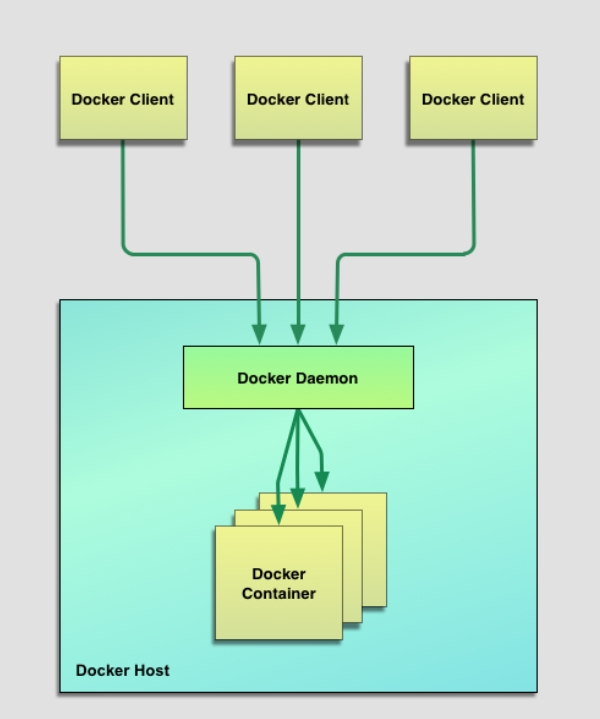
\includegraphics[width=0.9\textwidth]{./images/intro_dockerArchitecture.jpg}
          \caption{Die Client-Server-Architektur von Docker \cite{dockerUnderstandingDocker}.}
          \label{fig:intro_dockerArchitecture}
      \end{figure}

      Der Daemon kann von einer Registry Images (siehe Abschnitt \ref{dockerImages} und \ref{dockerRegistries}) beziehen, z.B. dem öffentlichen \emph{Docker Hub}.
      % Kommunikation zwischen Client und Server via TCPIP oder Unix Sockets?

      Der Docker-Host selbst ist wie in \fig \ref{fig:intro_dockerHost} dargestellt, aufgebaut. In einem Hostsystem läuft ein Linux-Betriebssystem, auf dem die Docker-Engine installiert ist. Die Engine verwaltet den Betrieb von Containern (siehe Abschnitt \ref{dockerContainer}), in denen in \fig \ref{fig:intro_dockerHost} die Applikationen A-E laufen. Wie auch in der Grafik zu sehen ist, teilen sich die Container gemeinsam verwendete Bibliotheken. Diese Eigenschaft wird in Abschnitt \ref{dockerImages} näher untersucht.

      \begin{figure}[h]
          \centering
          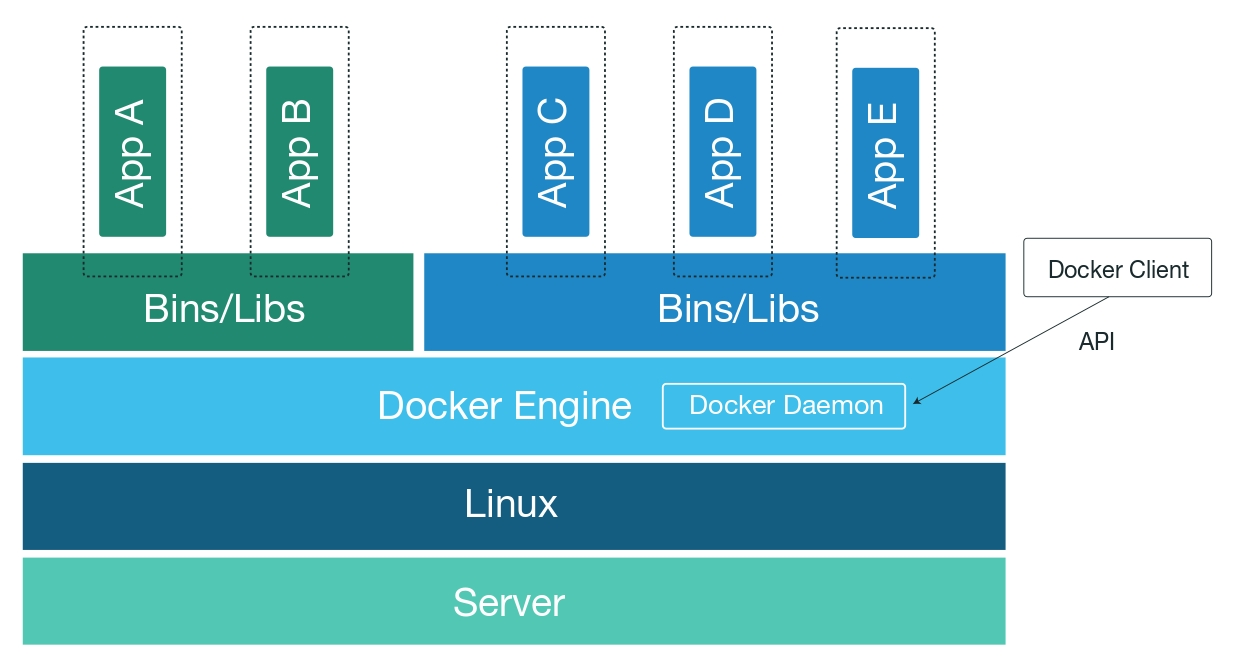
\includegraphics[width=0.9\textwidth]{./images/intro_dockerHost.jpg}
          \caption{Aufbau eines Docker"=Hostsystems \cite[S.3]{dockerSecIntro}.}
          \label{fig:intro_dockerHost}
      \end{figure}

		\subsection{Dockerfile}
		\label{dockerDockerfile}
      Ein Dockerfile ist eine Datei mit selbigem Namen, die die Erstellung eines Images mithilfe einer oder mehrerer Anweisungen spezifiziert. Anweisungen werden konsekutiv ausgeführt und führen jeweils zu einer neuen Schicht eines Images, die später in Summe das Image ergeben. Damit stellen Dockerfiles eine einfache Möglichkeit dar, Images auf Basis einer Vorlage automatisiert zu generieren.

			Eine Anweisung kann z.B. ein Tool installieren oder starten, eine Umgebungsvariable festgelegen oder einen Port öffnen. Ein exemplarisches Dockerfile ist im Folgenden dargestellt \cite{githubDockerfileNginx}.

			\begin{lstlisting}
				FROM ubuntu

				RUN \
					apt-get update && \
					apt-get install -y nginx

				WORKDIR /etc/nginx
				CMD ["nginx"]

				EXPOSE 80
				EXPOSE 443
			\end{lstlisting}

			Wie in diesem Dockerfile zu erkennen ist, bestehen Anweisungen aus einem Schlüsselwort in Großbuchstaben und mindestens einem Parameter. Die Erklärungen zu den einzelnen Anweisungen ist in Tabelle \ref{tab:dockerfile} gegeben \cite{dockerDockerfileDocs}:

			%\begin{itemize}
				%\item \texttt{FROM}: Setzt das Basisimage für alle folgenden Anweisungen. Jedes Dockerfile muss diese Anweisung am Anfang enthalten.
				%\item \texttt{RUN}: Führt angehängten Befehl während des \gls{Build}vorgangs aus. Mit \texttt{\&\&} können mehrere Befehle konsekutiv ausgeführt werden.
				%\item \texttt{WORKDIR}: Setzt das Arbeitsverzeichnis, von dem aus z.B. alle folgenden \texttt{RUN}- und \texttt{CMD}-Anweisungen ausgeführt werden. Kann mehrmals pro Dockerfile vorkommen.
				%\item \texttt{CMD}: Führt angehängten Befehl aus, wenn der Container gestartet wird. Pro Dockerfile kann es nur eine \texttt{CMD}-Anweisung geben.
				%\item \texttt{EXPOSE}: Öffnet angegebenen Port des Containers zur Laufzeit, in obigem Beispiel Port 80 und 443 für \acrshort{HTTP} und \acrshort{HTTPS}. Gebunden wird dieser standardmäßig auf dem Host auf einen \glqq{}registered\grqq{} Port (1024-49151).
			%\end{itemize}

			\vspace{0.5cm}
			\begin{table}[htp]
				\begin{centering}
				\begin{tabularx}{\textwidth}{>{\hsize=0.5\hsize}X|>{\hsize=1\hsize}X}
					\hline
					\textbf{Schlüsselwort} & \textbf{Bedeutung} \\
					\textbf{einer Anweisung} & \\
					\hline
					\texttt{FROM}
					& Setzt das Basisimage für alle folgenden Anweisungen. Jedes Dockerfile muss diese Anweisung am Anfang enthalten. In obigem Beispiel wird die neuste \emph{Ubuntu}-Version verwendet. \\
					\hline
					\texttt{RUN}
					& Führt den angehängten Befehl während des \gls{Build}vorgangs aus und erzeugt damit eine neue Schicht. \\
					\hline
					\texttt{WORKDIR}
					& Setzt das Arbeitsverzeichnis als Bezugspunkt für alle folgenden \texttt{RUN}- und \texttt{CMD}-Anweisungen. Kann mehrmals pro Dockerfile vorkommen. \\
					\hline
					\texttt{CMD}
					& Führt den angehängten Befehl aus, wenn der Container gestartet wird. Pro Dockerfile kann nur eine \texttt{CMD}-Anweisung existieren. \\
					\hline
					\texttt{EXPOSE}
					& Öffnet den angegebenen Port des Containers zur Laufzeit. In obigem Beispiel sind das Port 80 und 443 für \acrshort{HTTP} und \acrshort{HTTPS}. Auf dem Hostsystem werden diese standardmäßig auf einen Port zwischen 1024 und 49151 abgebildet. \\
					% \glqq{}registered\grqq{} Port ....
					\hline
				\end{tabularx}
				\vspace{0.5cm}
				\caption{Anweisungen eines Dockerfiles und deren Bedeutung.}
				\label{tab:dockerfile}
				\end{centering}
			\end{table}



		\subsection{Containerformate \emph{\acrshort{LXC}}, \emph{libcontainer} und \emph{\acrshort{OCF}}}
		\label{dockerContainerformate}
			Containerformate bilden das Herzstück der containerbasierten Virtualisierung. In ihnen ist in Form einer \acrshort{API} definiert, auf welche Art und Weise Container mit dem Hostsystem kommunizieren. Es wird z.B. festgelegt, wie das Dateisystem des Hostsystems verwendet wird, welche Features genutzt werden dürfen und wie die allgemeine Laufzeitumgebung von Containern spezifiziert ist.

			Dockers Containerformat hat sich in den letzten Monaten oft verändert, daher soll an dieser Stelle auf die neusten Entwicklungen eingegangen werden.

			Im ersten Release von Docker wurde die Ausführungsumgebung \emph{LXC} verwendet, die im März 2014 von der \emph{Docker}-eigenen Entwicklung \emph{libcontainer} abgelöst wurde. \emph{libcontainer} ist komplett in der Programmiersprache \emph{Golang} implementiert und kann ohne weitere Abhängigkeiten mit dem Linux-Kernel kommunizieren \cite{dockerLibcontainer}.

			Ende Juni 2015 kündigte Docker an, zusammen mit mehr als 20 Vertretern aus der Industrie, u.a. \emph{Google}, \emph{IBM} und \emph{VMware}, einen neuen Standard \emph{Open Container Format} (\emph{\acrshort{OCF}}) zu schaffen, welcher im Rahmen des \emph{Open Container Project}s (\emph{\acrshort{OCP}}) entstehen soll \cite{dockerOCP}. Gleichzeitig stellte \emph{\acrshort{runC}} vor, das eine Implementierung des \emph{OCF} darstellt und maßgeblich auf dem alten Format \emph{libcontainer} beruht \cite{dockerRunC}\cite{dockerRunCGithub}\cite{runC}.

		\subsection{Image}
    \label{dockerImages}
			Images bilden als unveränderbare Dateien die Basis von Containern. Sie sind einfach portierbar und können geteilt, gespeichert und aktualisiert werden. Images sind durch ein \emph{Union}-Dateisystem in Schichten unterteilt, die überlagert ein Image ergeben, das als Container gestartet werden kann \cite[S.11]{dockerBook}. Die von Docker unterstützten \emph{Union}-Dateisysteme, wie z.B. \emph{AuFS}, \emph{Brtfs} und \emph{Device Mapper} basieren auf dem \emph{\gls{CopyOnWrite}}-Modell \cite[S.8]{dockerBook}\cite[S.3]{dockerIntroIEEE}\cite[S.4]{dockerSecIntro}.
			% TODO: Zusatz: "Die Docker alle unterstuetzt (mit Storage Drivern)"

			Genauer gesagt besteht ein Image aus einem Manifest, das ein oder mehrere Schichten (Layers) referenziert. Images und Schichten sind jeweils über Hashwerte eindeutig referenzierbar und liegen auf dem Docker"=Hostsystem im Verzeichnis \texttt{/var/lib/docker/graph/}. Im Unterordner eines Images liegen mehrere, für ein Image spezifische Dateien (s. \fig \ref{fig:intro_dockerImageVZ}), u.a. das Manifest in der Datei \texttt{json}, das in einer \acrshort{JSON}-Struktur vorliegt und neben Metainformationen auch Details des Dockerfiles, aus dem das Image generiert wurde, beinhaltet \cite{githubDockerGlossary}.

			\begin{figure}[!htbp]
          \centering
          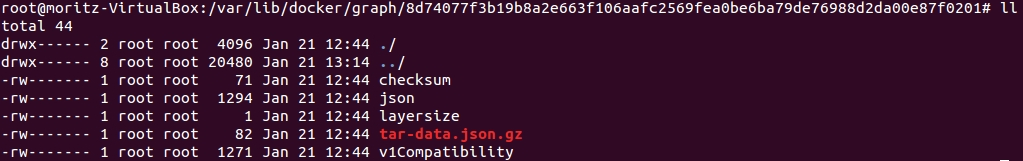
\includegraphics[width=1.0\textwidth]{./images/intro_dockerImageVZ.jpg}
          \caption{Dateien im Ordner eines Images (eigene Abbildung).}
          \label{fig:intro_dockerImageVZ}
      \end{figure}

			Images werden schrittweise aus den Anweisungen eines Dockerfiles erstellt. Die Schichten eines Images stellen i.d.R. eine minimale Ausführungsumgebung mit Bibliotheken, Binaries und Hilfspaketen sowie den Quellcode der Anwendung, die im Container ausgeführt werden soll, dar. Die Schichtenstruktur erlaubt es, Images modular aufzubauen, sodass sich Änderungen eines Images nur auf eine Schicht auswirken.

			Soll z.B. in ein bestehendes Image der Webserver \emph{Nginx} integriert werden, kann dieser mit dem Kommando \texttt{apt-get install nginx} innerhalb eines Containers zur Laufzeit installiert werden, was eine neue Schicht im Image zur Folge hat.

			Mit mehreren ähnlichen Images ist gewährleistet, dass nur die konkreten Unterschiede zwischen diesen als eigene Schichten hinterlegt sind. Eine gemeinsame Codebasis, die von mehreren Images genutzt wird, liegt in wenigen Schichten vor, die sich die Images teilen \cite[S.3]{dockerIntroIEEE}.

			Wie in \fig \ref{fig:intro_imagelayers} zu sehen ist, basieren die beiden beispielhaften Images \texttt{redis:3.0.6} und \texttt{nginx:1.9.9} auf zwei gleichen Schichten, die durch die Anweisungen \texttt{ADD} und \texttt{CMD} jeweils erzeugt werden. In dieser Abbildung sind die einzelnen Schichten eines Images vertikal gelistet. Merkmale der resultierenden Images sind in der ersten Zeile zusammengefasst.
      % Vergleich mit git commit und VCS (S.3 dockerIntroIEEE)

			\begin{figure}[!htbp]
          \centering
          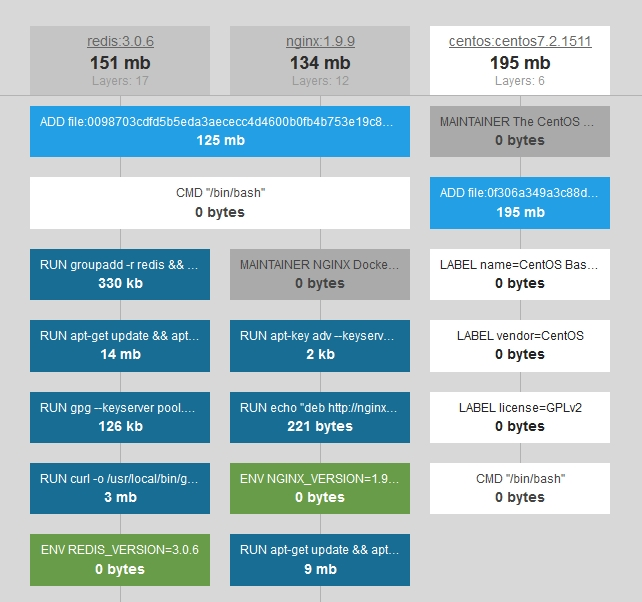
\includegraphics[width=0.9\textwidth]{./images/intro_imagelayers.jpg}
          \caption{Vergleich von drei Images auf Schichtebene \cite{dockerImagelayers}.}
          \label{fig:intro_imagelayers}
      \end{figure}

      % Copy-on-write erklären.

      Wie in \fig \ref{fig:intro_dockerPull} dargestellt, kann über die \gls{Shell} z.B. das Image eines \emph{CentOS}-Betriebssystems mit dem Befehl \texttt{docker pull nginx} aus dem \emph{Docker Hub} (siehe Abschnitt \ref{dockerRegistries}) bezogen werden \cite{dockerHubNginx}\cite{dockerPull}. Wie in \fig \ref{fig:intro_imagelayers} und \fig \ref{fig:intro_dockerPull} zu sehen ist, werden sechs Schichten heruntergeladen, die jeweils über einen Hashwert identifiziert werden und zusammengefügt das angefragte Image \texttt{centos:7.2.1511} ergeben.

			\begin{figure}[!htbp]
          \centering
          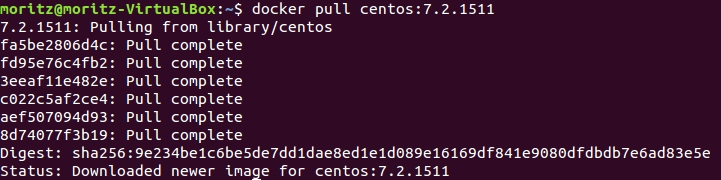
\includegraphics[width=1.0\textwidth]{./images/intro_dockerPull.jpg}
          \caption{Screenshot von der Ausführung des Befehls \texttt{docker pull IMAGE} (eigene Abbildung).}
          \label{fig:intro_dockerPull}
      \end{figure}

			Eine Liste aller lokal auf dem Hostsystem vorliegenden Images, kann - wie in \fig \ref{fig:intro_dockerImages} - mit dem Befehl \texttt{docker images} in der Shell generiert werden \cite{dockerImages}.

			\begin{figure}[!htbp]
          \centering
          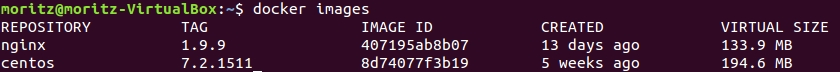
\includegraphics[width=1.0\textwidth]{./images/intro_dockerImages.jpg}
          \caption{Screenshot von der Ausführung des Befehls \texttt{docker images} (eigene Abbildung).}
          \label{fig:intro_dockerImages}
      \end{figure}

			% TODO: Ist Quelle https://docs.docker.com/engine/reference/commandline/images/ hier mit drin - eingearbeitet?

			% Seit registry api version 2 sind images content addressable
			%	Über kryptographisch sichere Hash ...sha256(bytes)
			% einfach und unabhängig verifizierbar
			% leverages merkle DAG ... damit naeher an git
			% weitere Vorteile auf s.21
			% unterschiede zu v1 auf s.23
			% seit docker 1.6 ist registrz v2 im einsatz
			%		^ 	\cite[S.15+16]{http://www.slideshare.net/Docker/docker-48351569}
			%

    \subsection{Container}
		\label{dockerContainer}
      % Metapher mit dem Docker-Wal, der Container lädt: Docker als Frachtschiff, mit dem Container verschifft werden.
			Ein Container ist die laufende Instanz eines Images, die in Sekundenbruchteilen startet \cite[S.1]{dockerIntroIEEE}. Er existiert als Gastsystem auf einem Docker"=Hostsystem und kann mehrere Anwendungen betreiben. Nach dem Konzept von \emph{Microservices} läuft in einem Container nur eine Anwendung.

      Ein Container wird über eine Reihe an Operationen gesteuert. Diese umfassen das Erstellen, Starten, Stoppen, Neustarten und Beenden eines Containers. Welchen Inhalt einen Container hat, also ob ein Container z.B. auf einem Datenbank- oder Webserver-Image beruht, ist dafür unerheblich \cite[S.12]{dockerBook}\cite[S.2]{dockerLXCKub}.

			Beispielsweise wird ein Container über das Kommando \texttt{docker run IMAGE} gestartet und über \texttt{docker rm CONTAINER} gestoppt.

			Wie in \fig \ref{fig:intro_dockerContainer} illustriert, wird dem Image beim Startvorgang eine weitere Containerschicht hinzugefügt, in die Datenänderungen während dem Containerbetrieb geschrieben werden. Auf die Schichten des unterliegenden Images wird nur lesend zugegriffen.

			\begin{figure}[!htbp]
          \centering
          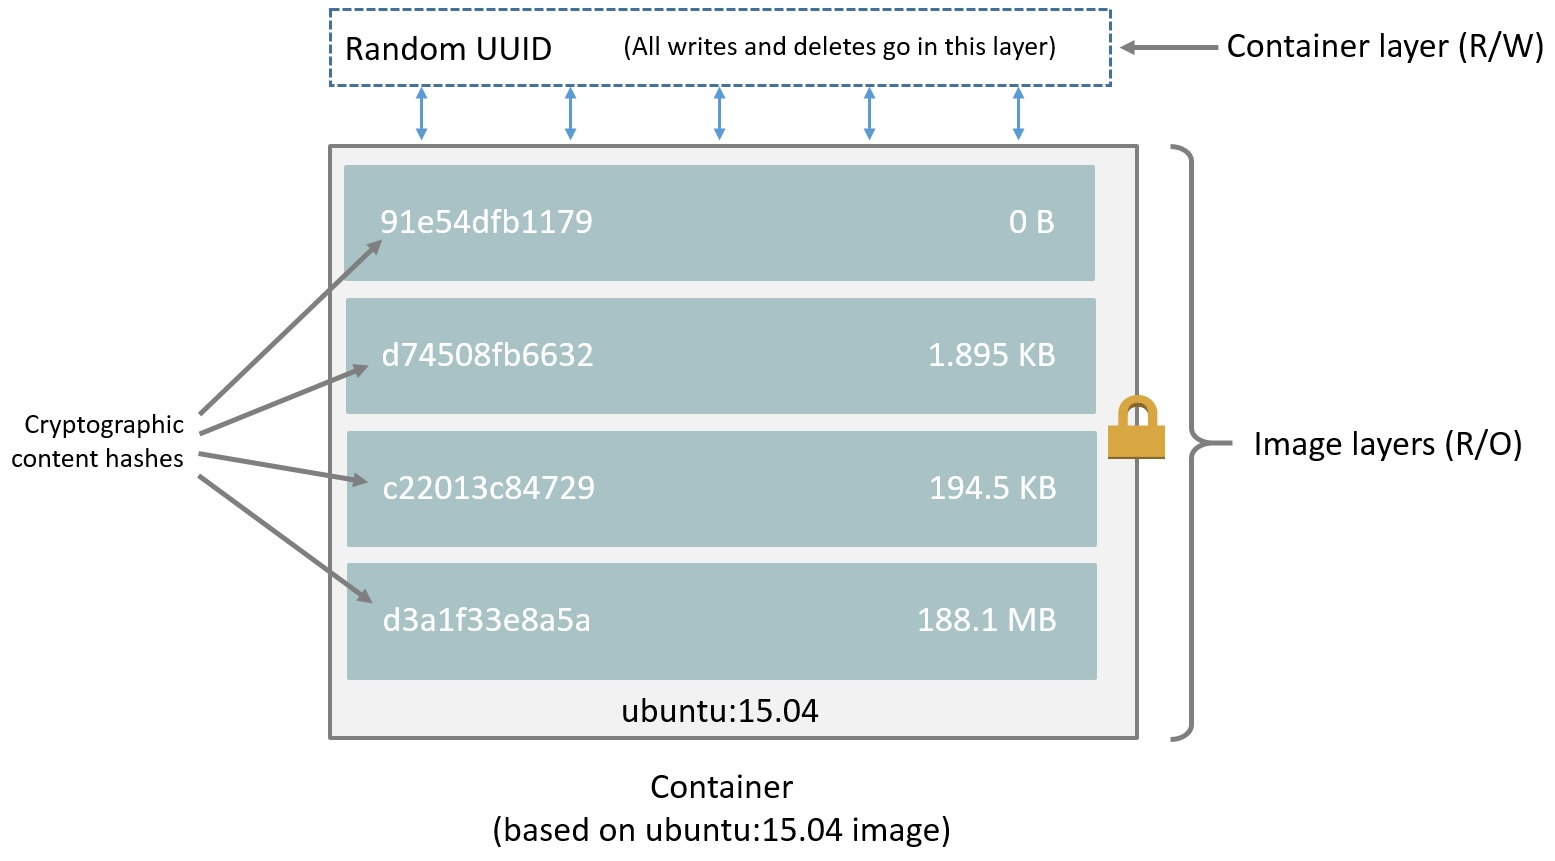
\includegraphics[width=1.0\textwidth]{./images/intro_dockerContainer.jpg}
          \caption{Schichtenaufbau eines Containers \cite{dockerImagesAndContainers}.}
          \label{fig:intro_dockerContainer}
      \end{figure}

      Ein Container wird als priveligiert bezeichnet, wenn er mit Rootrechten gestartet wurde. Standardmäßig startet ein Container unpriveligiert ohne Rootrechte. Mit einem reduzierten Set an ausführbaren Aktionen, die über verschiedenene, in Kapitel \ref{secLinux} vorgestellte Mechanismen definiert werden, lassen sich Container unabhängig von Rootrechten einschränken.
			% QUELLE + Verweis auf capabiltiies kapitel? Oder Glossareintrag "capabilities"

      % Der Hosts selbst muss auch gemanaged werden.
      % Docker als Anwendung muss installiert, gemanaged, und deployed werden auf einem Host.
      % Docker-Container müssen orchestriert, gemanged und deployed werden. Oft im Zusammenspiel mit externen Service und Tools.
      % In Hypervisor-basierten Virtualisierungen kommen meist Puppet, Chef )und Vagrant) zum Einsatz, die obigen Management-Anforderungen erfüllen können.
      % Aber beim Einsatz von Docker sind diese Tools nicht unbedingt notwendig,  Docker repräsentiert oft kurzlebige Container, read-only Container, die einfach zu ersetzen sind ohne die Notwendigkeit Containerzustände zu speichern oder wiederherzustellen. Wenn ein Zustand von Bedeutung ist, kann es einfacher sein diesen neu zu erstellen anstatt einen bestehnden Zustand zu korrigieren.
      % ^  \cite[S.14]{dockerBook}

      % In der Praxis werden herkömmliche, oft historisch gewachsene Lösungen nicht vollständig und sofort auf Docker umgerüstet. Mit der Koexistenz von Hypervisor-basierten Virtualisierungen und Containerlösungen, werden auch Configuration Management Tools wie Puppet und Chef im Zusammenhang mit Docker verwendet.
      % ^  \cite[S.14]{dockerBook}

		\subsection{Registry}
		\label{dockerRegistries}
      Eine Registry ist eine Webanwendung, die als Speicher- und Verteilerplattform für Images dient. Über eine Registry-API sind Docker-Komponenten in der Lage, mit Registries zu kommunizieren. Images sind mit Tags versehen in Repositories gegliedert, die wiederum in der Registry persistiert werden \cite{dockerRegistry}. %Ein Repository besteht aus mindestens einem Image.
			% (TODO): visit source, and extend registry info here
			% (TODO): was zu registry api version 1 und 2, 2.1, 2.2, 2.3 schreiben und bisschen vergleichen
			%		^		\cite{http://www.slideshare.net/Docker/docker-48351569 ... slide 11}\cite{https://docs.docker.com/registry/spec/api/}

      \emph{Docker} stellt eine Vielzahl an Images frei verfügbar über einen Dienst, dem \emph{Docker Hub}, zur Verfügung \cite[S.11]{dockerBook}\cite[S.3]{dockerSec1}\cite{dockerRegistry}. Für dieses System können Personen und Organisationen Konten anlegen und eigenständig Images in öffentliche und private Repositories hochladen. Das \emph{Docker Hub} bietet bereits mehr als 150.000 Repositories, die von ca. 240.000 Nutzern zusammengestellt und hochgeladen wurden (Stand: Juni 2015) \cite[S.16]{slideshareDockercon15}. Wie in \fig \ref{fig:intro_registry} zu sehen ist, werden auch Nutzungsstatistiken pro Image gesammelt und angezeigt. Durch diese erweiternden Features ist das \emph{Docker Hub} strenggenommen keine Registry, sondern enthält eine Registry als Teil einer Webanwendung. % \cite[S.8]{http://www.slideshare.net/Docker/docker-48351569}

      \begin{figure}[h]
          \centering
          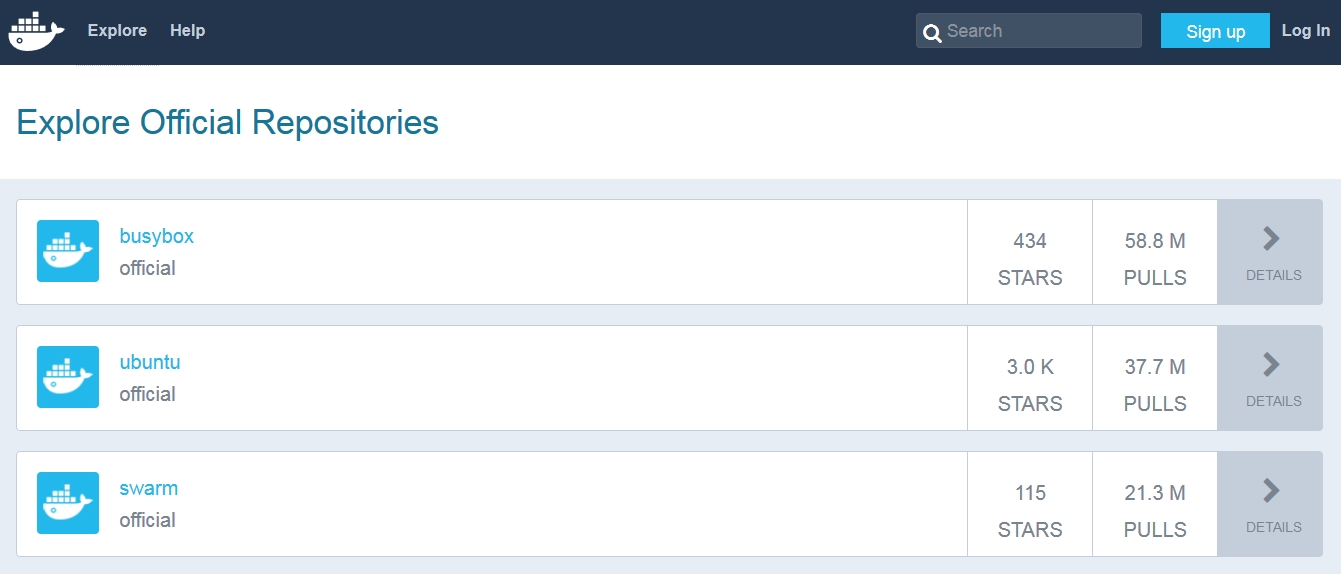
\includegraphics[width=1.0\textwidth]{./images/intro_registry.jpg}
          \caption{Web-\acrshort{UI} des Docker Hubs mit den beliebtesten Repositories \cite{dockerHub}.}
          \label{fig:intro_registry}
      \end{figure}

			Um Images in einem Repository voneinander zu unterscheiden, werden diese mit sogenannten Tags gekennzeichnet, um mehrere Versionen eines Images in einem Repository zu markieren. Die Images werden nach dem Schema \texttt{<repository>:<tag>} identifiziert. Es gibt z.B. im offiziellen Repository des Webservers \emph{Nginx} mehrere Images mit den Tags \texttt{latest}, \texttt{1}, \texttt{1.9} und \texttt{1.9.9} \cite{dockerHubNginx}.
			%Wenn beim Herunterladen kein Tag angegeben ist, wird automatisch die aktuellste Imageversion mit dem Tag \texttt{latest} bezogen.

      % es gibt eine Trusted Registry. Die noch erklären.

      % Bsp. geben für z.B. Ubuntu mit vielen Unterversionen und dem Identifier "latest".

      % Weitere beispiele aus dockerBook: Nginx web server, MySQL Datenbank

      % Es gibt offizielle Images, die von trusted parties verwaltet werden

\end{document}
